% Template file for an a0 portrait poster.
% Written by Graeme, 2001-03 based on his SOC poster.
%
% See discussion and documentation at
% <http://www.astro.gla.ac.uk/users/norman/docs/posters/> 
%
%%%%%%%%%%%%%%%%%%%%%%%%%%%%%%%%%%%%%%%%
% Modified by Jozef Dobo\v{s} (c) 2011 % 
%%%%%%%%%%%%%%%%%%%%%%%%%%%%%%%%%%%%%%%%

\documentclass[a1,portrait]{a1poster}
% You might find the 'draft' option to a0 poster useful if you have
% lots of graphics, because they can take some time to process and
% display. (\documentclass[a0,draft]{a0poster})

\pagestyle{empty}
\setcounter{secnumdepth}{0}
\usepackage[absolute]{textpos}
\usepackage{wrapfig,times}
\usepackage{graphicx}
\usepackage{forloop}
\usepackage[margin=0cm]{geometry}
%\usepackage{framed,color}
\usepackage{tikz}
\usetikzlibrary{shapes,snakes}
\usepackage{setspace}
\usepackage{bm}
\usepackage[varg]{txfonts}
\usepackage{rotating}
\usepackage{comment} 

\usepackage{color}
\usepackage[colorlinks, pdfborder={0 0 0}]{hyperref}
\definecolor{LinkColor}{rgb}{0.75, 0, 0}
\definecolor{CiteColor}{rgb}{0, 0.5, 0.5}
\definecolor{UrlColor}{rgb}{0, 0, 0.75}
\hypersetup{linkcolor=LinkColor}
\hypersetup{citecolor=CiteColor}
\hypersetup{urlcolor=UrlColor}
\DeclareMathAlphabet{\mathpzc}{OT1}{pzc}{m}{it}



%%%%%%%%%%
% Colors %
%%%%%%%%%%
\usepackage{color}
\definecolor{TitleColor}{rgb}{1,1,1} % white
\definecolor{BannerOneColor}{rgb}{0,0,0} % pitch black
\definecolor{BannerTwoColor}{rgb}{0.93,0.08,0.31} % pinky red
\definecolor{BannerThreeColor}{rgb}{0,0.27,0.48} % dark blue
\definecolor{BannerFourColor}{rgb}{0.33,0.19,0.098} % brown
\definecolor{BannerFiveColor}{rgb}{.93,0.,0.03} % some shade in red
\definecolor{BannerSixColor}{rgb}{0,0.27,0.42} % dark blue
\definecolor{BannerSevenColor}{rgb}{0.62,0.77,0.86} % sky blue
\definecolor{BannerEightColor}{rgb}{0.35,0.33,0.01} % military green
\definecolor{BannerNineColor}{rgb}{0.85,0.86,0.34} % lime green
\definecolor{BannerTenColor}{rgb}{0,0.66,0.80} % strong blue
\definecolor{BannerElevenColor}{rgb}{0.46,0,0.20} % maroon
\definecolor{BannerTwelveColor}{rgb}{0.37,0.32,0.44} % dark washed violet
\definecolor{BannerThirteenColor}{rgb}{0.79,0.84,0.65} % light washed green
\definecolor{BannerFourteenColor}{rgb}{0.57,0.64,0.27} % dark washed green
\definecolor{BannerFifteenColor}{rgb}{0.92,0.91,0.88} % unusable washed 
\definecolor{BannerSixteenColor}{rgb}{0.97,0.36,0.14} % strong orange
\definecolor{BannerSeventeenColor}{rgb}{0.97,0.61,0.19} % orange
\definecolor{BannerEighteenColor}{rgb}{0.99,0.76,0.11} % mustard yellow
\definecolor{BannerNineteenColor}{rgb}{0.79,0.76,0.73} % light gray-ish
\definecolor{BannerTwentyColor}{rgb}{0.63,0.58,0.54} % dark gray-ish

\definecolor{shadecolor}{rgb}{0.92,0.91,0.88} % unusable washed 
%%%%%%%%%%%%%%%%%%%%%%%%%%%%%%%%%%%%%%%%%%%%%%%%%%%%%%
% Only change here to affect all headings            %
\newcommand{\headingcolor}{\color{BannerElevenColor}} 
\newcommand{\red}[1]{{\textcolor{red} {{#1}}}} 
\newcommand{\ajith}[1]{{\textcolor{magenta} {\textit{Ajith: #1}}}} 
\newcommand{\aditya}[1]{{\textcolor{magenta} {\textit{Aditya: #1}}}}
\newcommand{\sumit}[1]{{\textcolor{magenta} {\textit{Sumit: #1}}}}
\newcommand{\saketh}[1]{{\textcolor{magenta} {\textit{Saketh: #1}}}}
\newcommand{\x}{\mathbf{x}}
\newcommand{\y}{\mathbf{y}}
\newcommand{\ba}{\mathbf{a}}
\newcommand{\bb}{\mathbf{b}}
\newcommand{\br}{\mathbf{r}}
\newcommand{\xprime}{\mathbf{x^\prime}}
\newcommand{\xiin}{\xi_\mathrm{in}}
\newcommand{\xit}{\xi_\mathrm{tr}}
\newcommand{\xis}{\xi_\mathrm{sm}}
\newcommand{\xisdm}{\xi_\mathrm{sm}^\mathrm{DM}}
\newcommand{\xiproc}{\xi_\mathrm{proc}}
\newcommand{\bmu}{\bm \mu}
\newcommand{\bal}{\bm \alpha}
\newcommand{\bnu}{\bm \nu}
\newcommand{\Pt}{P_\mathrm{tr}}
\newcommand{\dt}{d_\mathrm{tr}}
\newcommand{\C}{\mathsf{C}}
\newcommand{\CS}{\mathsf{C'}}
\newcommand{\N}{\mathcal{N}}
\newcommand{\ddelta}{\delta^{(3)}}


%%%%%%%%%%%%%%%%%%%%%%%%%%%%%%%%%%%%%%%%%%%%%%%%%%%%%%

% see documentation for a0poster class for the size options here
%\let\Textsize\normalsize
\let\Textsize\Large
\def\Head#1{\noindent\hbox to \hsize{\hfil{\LARGE \headingcolor #1}}\bigskip}
\def\LHead#1{\noindent{\LARGE \headingcolor #1}\smallskip}
\def\Authors#1{\noindent{\large#1}\smallskip}
\def\Subhead#1{\noindent{\large \headingcolor #1}}
\def\Title#1{\noindent{\huge #1}}

% define the color of the emphasis text here. Please use a text color 
% consistent with the color scheme of the poster 
\def\emphasis#1{{\large \color{BannerTwoColor} {#1}}}	

% Set up the grid
%
% Note that [0cm,0cm] is the margin round the edge of the page --
% it is _not_ the grid size. That is always defined as 
% PAGE_WIDTH/HGRID and PAGE_HEIGHT/VGRID. In this case we use
% 25 x 25. This gives us three wide columns for text (7 grid
% spacings) and four narrow columns (1 each) at each side of these 
% text columns
%
% Note however that texblocks can be positioned fractionally as well,
% so really any convenient grid size can be used.
%

% [margin, margin]{rows}{cols}
\TPGrid[0cm,0cm]{17}{25}  % 1 - 7 - 1 - 7 - 1 Columns


% Mess with these as you like
\parindent=0pt
%\parindent=1cm
\parskip=0.5\baselineskip
\linespread{1.1}

% abbreviations
\newcommand{\ddd}{\,\mathrm{d}}

\begin{document}

% Understanding textblocks is the key to being able to do a poster in
% LaTeX. In
%
%    \begin{textblock}{width}(x,y)
%    ...
%    \end{textblock}
%
% the first argument gives the block width in units of the grid
% cells specified above in \TPGrid; the second gives the (x,y)
% position on the grid, with the y axis pointing down.

%%%%%%%%%%%%%%
% Top Banner %
%%%%%%%%%%%%%%
% if you change this part, you can get matching color for headings
% in Colors section above


\begin{textblock}{25}(0,0)
%\includegraphics[width=\paperwidth]{banners/banner11.pdf}
\colorbox{BannerElevenColor}{\parbox[c][0.062\textwidth][c]{1.0\textwidth}{\rule{\linewidth}{0pt}}}
%\includegraphics[height=2.6in]{banners/banner11.pdf}
\end{textblock}




%%%%%%%%%%%%%%%%%%%%%%%%%%%%%%%%%%%%%%%%%%%%%%%%%%%%%%%%%%%%%%%%%%%%%%%%%
%%%%%%%%%%%%%%%%%%%%%%%%%%%%%%%%%% Title %%%%%%%%%%%%%%%%%%%%%%%%%%%%%%%%
%%%%%%%%%%%%%%%%%%%%%%%%%%%%%%%%%%%%%%%%%%%%%%%%%%%%%%%%%%%%%%%%%%%%%%%%%
\begin{textblock}{15}(0.75,0.1)	 % syntax: {colum_width} (x_coordinate, y_coordinate)
{\color{TitleColor}

\Title{\begin{center}
		Probing large scale structure with gravitational wave observations of binary black holes [arXiv:2005.01111]
	\end{center}}
}
\end{textblock}

\begin{textblock}{23}(0.75,1.88)
\Authors{\textbf{Aditya Vijaykumar}$^1$, ~MV Saketh$^2$, ~Sumit Kumar$^3$,  ~Parameswaran Ajith$^{1,4}$, ~Tirthankar Roy Choudhury$^{5}$} \\ 
\textit{$^1$ International Centre for Theoretical Sciences, Tata Institute of Fundamental Research, Bengaluru 560089, India} \\
\textit{$^{2}$ Department of Physics, University of Maryland, College Park, Maryland 20742, USA} \\
\textit{$^{3}$ Max-Planck-Institut f$\ddot{u}$r Gravitationsphysik (Albert-Einstein-Institut), D-30167 Hannover, Germany } \\
\textit{$^{4}$ Canadian Institute for Advanced Research,CIFAR Azrieli Global Scholar, MaRS Centre, West Tower, 661 University Ave, Toronto, ON M5G 1M1, Canada} \\
\textit{$^{5}$ National Centre for Radio Astrophysics, Tata Institute of Fundamental Research, Pune, India} \\
\end{textblock}
%%%%%%%%%%%%%%%%%%%%%%%%%%%%%%%%%%%%%%%%%%%%%%%%%%%%%%%%%%%%%%%%%%%%%%%%%


%%%%%%%%%%%%%%%%%%%%%% An example text block %%%%%%%%%%%%%%%%%%%%%%%%%%%%
%%%%%%%%%%%%%%%%%%%%%%%%%%%%%%%%%%%%%%%%%%%%%%%%%%%%%%%%%%%%%%%%%%%%%%%%%
%\begin{textblock}{7}(1,4.3)  
% syntax: {colum_width} (x_coordinate, y_coordinate) in inches
% Please do not change the column_width and x_coordinate
  %\LHead{Introduction}
%\begin{spacing}{3}
%\emphasis{Third generation gravitational-wave (GW) detectors are expected to detect a large number of binary black holes (BBHs) to large redshifts, opening up an independent probe of the large scale structure using their clustering. This probe will be complementary to the probes using galaxy clustering. We explore the possibility of probing the large scale structure from the spatial distribution of the observed BBH population, using their two-point (auto)correlation function. We find that we can estimate the bias factor of population of BBH (up to $z \sim 1$) with a few years of observations with these detectors. Our method relies solely on the source-location posteriors obtained from the GW events and does not require any information from electromagnetic observations. This will help in identifying the type of galaxies that host the BBH population, thus shedding light on their origins.}
%\end{spacing}

%\end{textblock}
%%%%%%%%%%%%%%%%%%%%%%%%%%%%%%%%%%%%%%%%%%%%%%%%%%%%%%%%%%%%%%%%%%%%%%%%%
%%%%%%%%%%%%%%%%%%%%%% An example text block %%%%%%%%%%%%%%%%%%%%%%%%%%%%
%%%%%%%%%%%%%%%%%%%%%%%%%%%%%%%%%%%%%%%%%%%%%%%%%%%%%%%%%%%%%%%%%%%%%%%%%

\begin{textblock}{7.3}(0.7,4.3)	% syntax: {colum_width} (x_coordinate, y_coordinate) in inches
\LHead{Introduction}\\
Future gravitational-wave detectors will detect \textbf{hundreds of thousands of BBH events a year}. We can imagine these events as a \textit{survey of BBHs}, akin to \textit{galaxy surveys}.

\begin{figure}
	\centering
	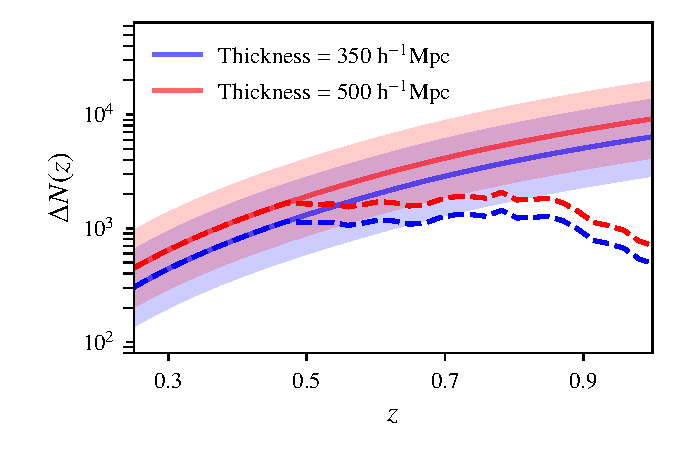
\includegraphics[scale=1.8]{Nz_vs_z.pdf}
	\caption{\small{Solid curve with shaded region shows the total number of detectable merger events as a function of redshift in shell of thickness $\sim 350~h^{-1}$~Mpc and $\sim 500~h^{-1}$~Mpc in comoving distance. The dashed lines show the average number of mergers in the shell of given thickness for which the errors in sky localization are within a degree square and errors in estimating the comoving distance are $\le 90~h^{-1}$~Mpc for a network of three 3G detectors.}} 
	\label{fig:mergers_events}
\end{figure}
Galaxy surveys can be used to measure the \textbf{two-point correlation function (2PCF)}. Given a cosmological density field $ \rho(x) $, one can define overdensity field $\delta(x) := \rho(x) / \overline{\rho} - 1$.
The 2PCF is  then given by
\begin{equation}
\xi({r}) = \left<\delta(\x) \, \delta(\y)\right> \label{corrfunc},
\end{equation}
where angle brackets denote the ensemble average. Assuming standard $ \Lambda $CDM cosmology, \textbf{we can calculate the 2PCF for dark matter $ \xi_{DM} $ theoretically}.\\

\LHead{The Linear Bias Factor}\\
Since dark matter is more abundant than the baryonic matter, the clustering of the galaxies is expected to trace that of the dark matter.
\begin{equation}
\xi_\mathrm{gal}(r) = b_\mathrm{gal}^2 \, \xi_\mathrm{DM}(r),
\end{equation}
$b_\mathrm{gal}$ is called the \textbf{linear bias}  and depends on the luminosity and color type of galaxies. Similarly, we can also define a \textbf{bias which quantifies the clustering of the observed BBH population}:
\begin{equation}
\xi_\mathrm{BBH}(r) = b_\mathrm{BBH}^2 \, \xi_\mathrm{DM}(r). 
\end{equation}

\LHead{Localization errors and $ \xi(r) $}
\begin{figure*}[t]
	\centering
	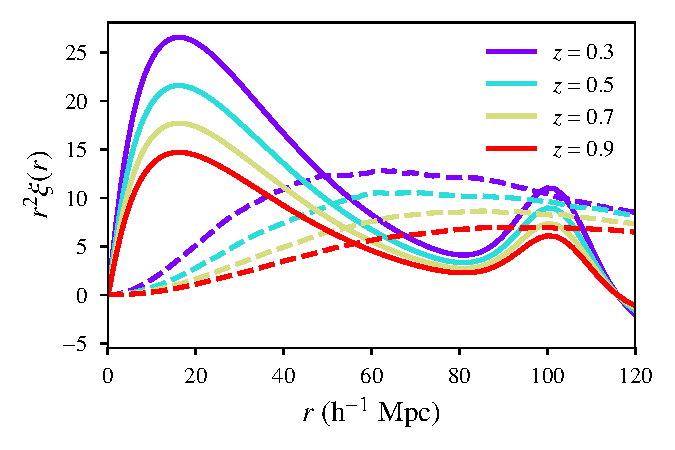
\includegraphics[scale=1.75]{processed_correlation_function.pdf}
	%\includegraphics[scale=1.2]{../../papers/HigherModes/figs/PNNRMatching_SpEC_q8.pdf}
	\caption{\small{The ``smeared'' correlation function (dashed lines) and the ``true'' correlation function (solid lines) for various redshifts. The true correlation function is simply the dark matter correlation function assuming the standard model of cosmology. The ``smearing'' is calculated assuming that the distribution of errors in localization of GW population follow a Gaussian distribution with mean $\{\mu_\mathrm{RA} = 0.5^\circ, \mu_\mathrm{dec} = 0.5^\circ, \mu_\mathrm{d} = 50~h^{-1}~\mathrm{Mpc}\}$ and standard deviation $\{\sigma_\mathrm{RA} = 0.5^\circ, \sigma_\mathrm{dec} = 0.5^\circ, \sigma_\mathrm{d} = 20 h^{-1}~\mathrm{Mpc}\}$. }}
	\label{fig:hybridTD_l2m2}
\end{figure*}


\end{textblock}

\begin{textblock}{7.3}(8.9,3.6)	% syntax: {colum_width} (x_coordinate, y_coordinate) in inches
\vspace{2cm}
Due to the large statistical uncertainties in the GW localization, \textbf{the observed correlation function of BBHs will smeared}. The smeared correlation function can be computed by convolving the actual correlation function $ \xi_\mathrm{tr} $ with the localization posteriors $ P(\x) $ obtained from GW data.
\begin{equation}
\xi(\x, \y) = \int_V dV_\mu \int_V dV_\nu \,  P(\x-\bmu) \, P(\y-\bnu) \, \xit(\bmu, \bnu)
\label{eq:xi_v2}
\end{equation}

\LHead{Simulations and Results}\\
\begin{figure}[t]
	\centering
	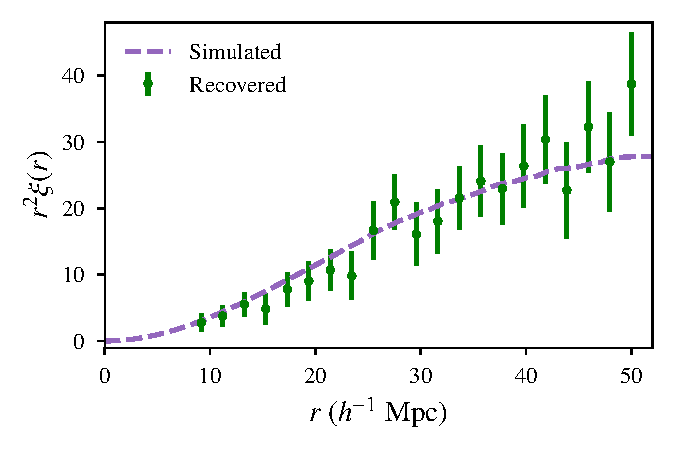
\includegraphics[scale=1.8]{comparison_data_expected.pdf}
	\caption{\small{Simulated (smeared) correlation function for a given distribution of localization errors is plotted along with the one recovered from simulated events at redshift 0.3 and input bias factor of 1.5. Smeared correlation function is scaled with input bias for comparison. We used 5000 simulated events distributed in a shell of thickness 350 $h^{-1}$~Mpc around redshift $0.3$} }
	\label{fig:simulation_example}
\end{figure}
We use the publicly available code \textsc{lognormal\_galaxies}\footnote{hello}, to simulate galaxy catalogs at various redshifts with a certain bias $ b_\mathrm{gal} $. We assume that GW events occur in any random subsample of the galaxies in the catalog, which essentially implies $b_\mathrm{BBH}=b_\mathrm{gal}$. We then simulate mock BBH catalogs by assuming a (gaussian) localization error distribution and check whether we are able to recover the bias consistent with the input value.\\

\begin{figure*}[t]
	\centering
	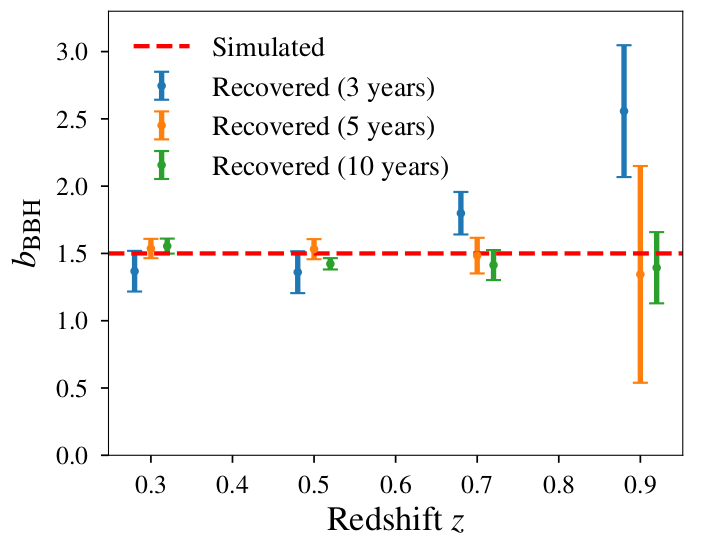
\includegraphics[scale=0.73]{moneyplot.png}
	%\includegraphics[scale=1.2]{../../papers/HigherModes/figs/PNNRMatching_SpEC_q8.pdf}
	\caption{\small{The recovered bias factor $b_\mathrm{BBH}$ ({68\%} confidence regions) from various redshifts bins (with shell thickness of $\sim 350~h^{-1}$ Mpc). The catalogs were created using the dark matter correlation function with  linear bias $1.5$. With a moderate observational time of three years, \textbf{we can recover the bias to within $\sim 20\%$ at $z \lesssim 0.7$, while errors in bias recovery are larger at redshift $z \sim 1$ due to large errors in localization}}}
\end{figure*}
The measured bias factor \textbf{probes the spatial distribution} of BBH mergers. It can be:
\begin{itemize}
	\item compared to the clustering properties of the galaxies as measured from the optical surveys  and obtain \textbf{insights on the type of galaxies that host these merger events}
	\item related to the \textbf{mass of dark matter halos these events reside in}
	\item used to to understand the \textbf{formation channels of the BBHs}.
\end{itemize}
\end{textblock}

%%%%%%%%%%%%%%%%%%%%%%%%%%%%%%%%%%%%%%%%%%%%%%%%%%%%%%%%%%%%%%%%%%%%%%%%%
%%%%%%%%%%%%%% Place the institute logos at the bottom left %%%%%%%%%%%%
%%%%%%%%%%%%%%%%%%%%%%%%%%%%%%%%%%%%%%%%%%%%%%%%%%%%%%%%%%%%%%%%%%%%%%%%%
\begin{textblock}{18}(9.,24.3)   
	\small{$^1$ - https://bitbucket.org/komatsu5147/lognormal\_galaxies/}
%\resizebox{2\TPHorizModule}{!}{\includegraphics{figs/icts_logo.pdf}} \hspace{1.cm}
%\resizebox{2\TPHorizModule}{!}{\includegraphics{figs/IndigoLogo_crop.png}} \hspace{1.cm}
%\resizebox{0.85\TPHorizModule}{!}{\includegraphics{figs/CardiffLogo.png}} \hspace{1.cm}
%\resizebox{0.85\TPHorizModule}{!}{\includegraphics{figs/logo-UIB.pdf}}
%\resizebox{1\TPHorizModule}{!}{\includegraphics{figs/rri-logo.jpg}}\hspace{1cm}
%\resizebox{1\TPHorizModule}{!}{\includegraphics{figs/cmi-header2.png}}
\end{textblock}
%%%%%%%%%%%%%%%%%%%%%%%%%%%%%%%%%%%%%%%%%%%%%%%%%%%%%%%%%%%%%%%%%%%%%%%%%

%%%%%%%%%%%%%%%%%%%%%%%%%%%%%%%%%%%%%%%%%%%%%%%%%%%%%%%%%%%%%%%%%%%%%%%%%
%%%%%%%%%%%%%%%%%%%%%%%%%%%% Acknowledgments %%%%%%%%%%%%%%%%%%%%%%%%%%%%
%%%%%%%%%%%%%%%%%%%%%%%%%%%%%%%%%%%%%%%%%%%%%%%%%%%%%%%%%%%%%%%%%%%%%%%%%

%%%%%%%%%%%%%%%%%%%%%%%%%%%%%%%%%%%%%%%%%%%%%%%%%%%%%%%%%%%%%%%%%%%%%%%%%


\end{document}

